%% LaTeX-Beamer template for KIT design
%% by Erik Burger, Christian Hammer
%% title picture by Klaus Krogmann
%%
%% version 2.1
%%
%% mostly compatible to KIT corporate design v2.0
%% http://intranet.kit.edu/gestaltungsrichtlinien.php
%%
%% Problems, bugs and comments to
%% burger@kit.edu

\documentclass[18pt]{beamer}

\usepackage[utf8]{inputenc}
\usepackage[babel,german=quotes]{csquotes}
\usepackage{graphicx}
\usepackage{caption}
\usepackage{subfig}
\usepackage[right]{eurosym}
\usepackage{listings}

%% SLIDE FORMAT

% use 'beamerthemekit' for standard 4:3 ratio
% for widescreen slides (16:9), use 'beamerthemekitwide'

\usepackage{templates/beamerthemekit}
% \usepackage{templates/beamerthemekitwide}

%% TITLE PICTURE

% if a custom picture is to be used on the title page, copy it into the 'logos'
% directory, in the line below, replace 'mypicture' with the 
% filename (without extension) and uncomment the following line
% (picture proportions: 63 : 20 for standard, 169 : 40 for wide
% *.eps format if you use latex+dvips+ps2pdf, 
% *.jpg/*.png/*.pdf if you use pdflatex)

\titleimage{title}

%% TITLE LOGO

% for a custom logo on the front page, copy your file into the 'logos'
% directory, insert the filename in the line below and uncomment it

\titlelogo{titlelogo}

% (*.eps format if you use latex+dvips+ps2pdf,
% *.jpg/*.png/*.pdf if you use pdflatex)

%% TikZ INTEGRATION

% use these packages for PCM symbols and UML classes
% \usepackage{templates/tikzkit}
% \usepackage{templates/tikzuml}

% the presentation starts here

\title[C++ Workshop]{C++ Workshop}
\subtitle{6. Block, 08. Juni 2012}
\author{Oliver Schneider, Robert Schneider}

\institute{}

\begin{document}

% change the following line to "ngerman" for German style date and logos
\selectlanguage{ngerman}

\AtBeginSection[]{%
	\begin{frame}
		\tableofcontents[sectionstyle=show/hide,subsectionstyle=hide/show/hide]
	\end{frame}
	\addtocounter{framenumber}{-1}% If you don't want them to affect the slide number
}

%title page
\begin{frame}
\titlepage
\end{frame}

%table of contents
\begin{frame}{Gliederung}
\tableofcontents
\end{frame}

%%%%%%%%%%%%%%%%%%%%%%%%%
% ADD OWN SECTIONS HERE %
%%%%%%%%%%%%%%%%%%%%%%%%%
\section{friendship}





\subsection{access modifiers}

\begin{frame}[fragile]{access modifiers}
	Wir kennen bereits für die member von Klassen (\verb|class|, \verb|struct|, \verb|union|).
	Wenn man sagt, eine Klasse habe Zugriff auf einen member, so bedeutet dies, dass die member dieser Klasse diesen Zugriff besitzten (z.B. member functions).
	
	\pause
	
	\begin{block}{Zugriffskontrolle für member}
		Zugriff für member in einer Klasse A für:
		\begin{itemize}[<+->]
			\item \verb|public| -- jeden
			\item \verb|protected| -- nur die Klasse A selbst und deren Kindklassen
			\item \verb|private| -- nur die Klasse A selbst
		\end{itemize}
	\end{block}
\end{frame}


\begin{frame}{encapsulation \& information hiding}
	\begin{itemize}[<+->]
		\item Faustregel: Alles so weit wie möglich schützen!
		\item data member i.d.R. private
		\item nur sichere, in sich geschlossene Funktionen public
	\end{itemize}
\end{frame}


\begin{frame}{friendship}
	Friendship erlaubt eine feinere Kontrolle über member access:
	
	\vspace{1em}
	
	\onslide*<+> { 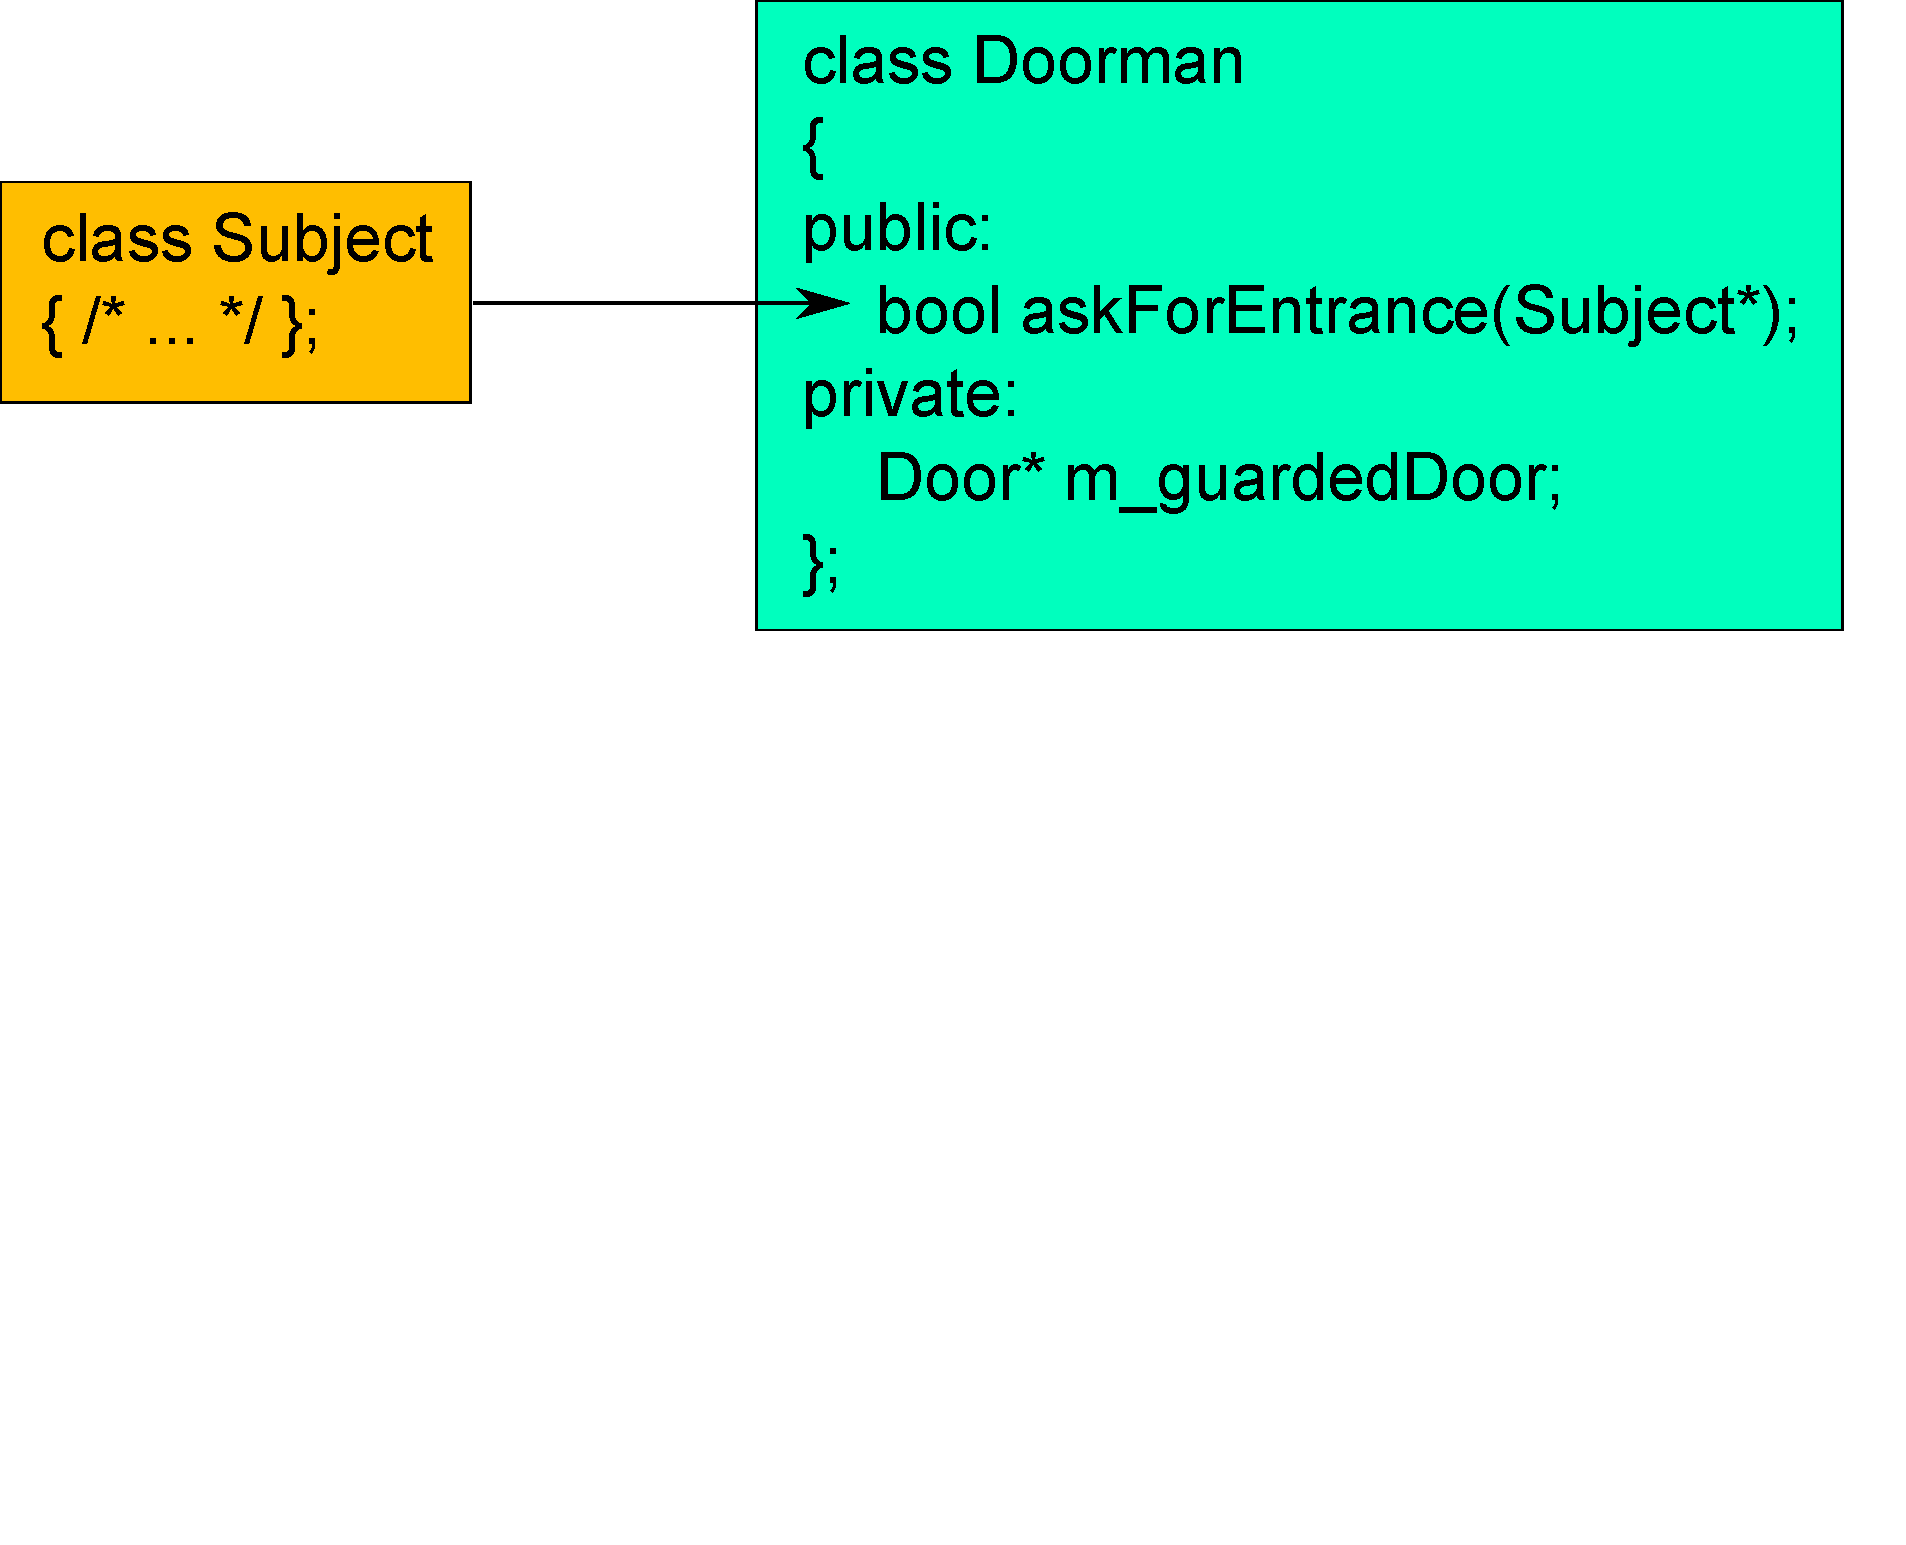
\includegraphics[height=0.75\textheight]{images/without-friendship-0} }
	\onslide*<+> { 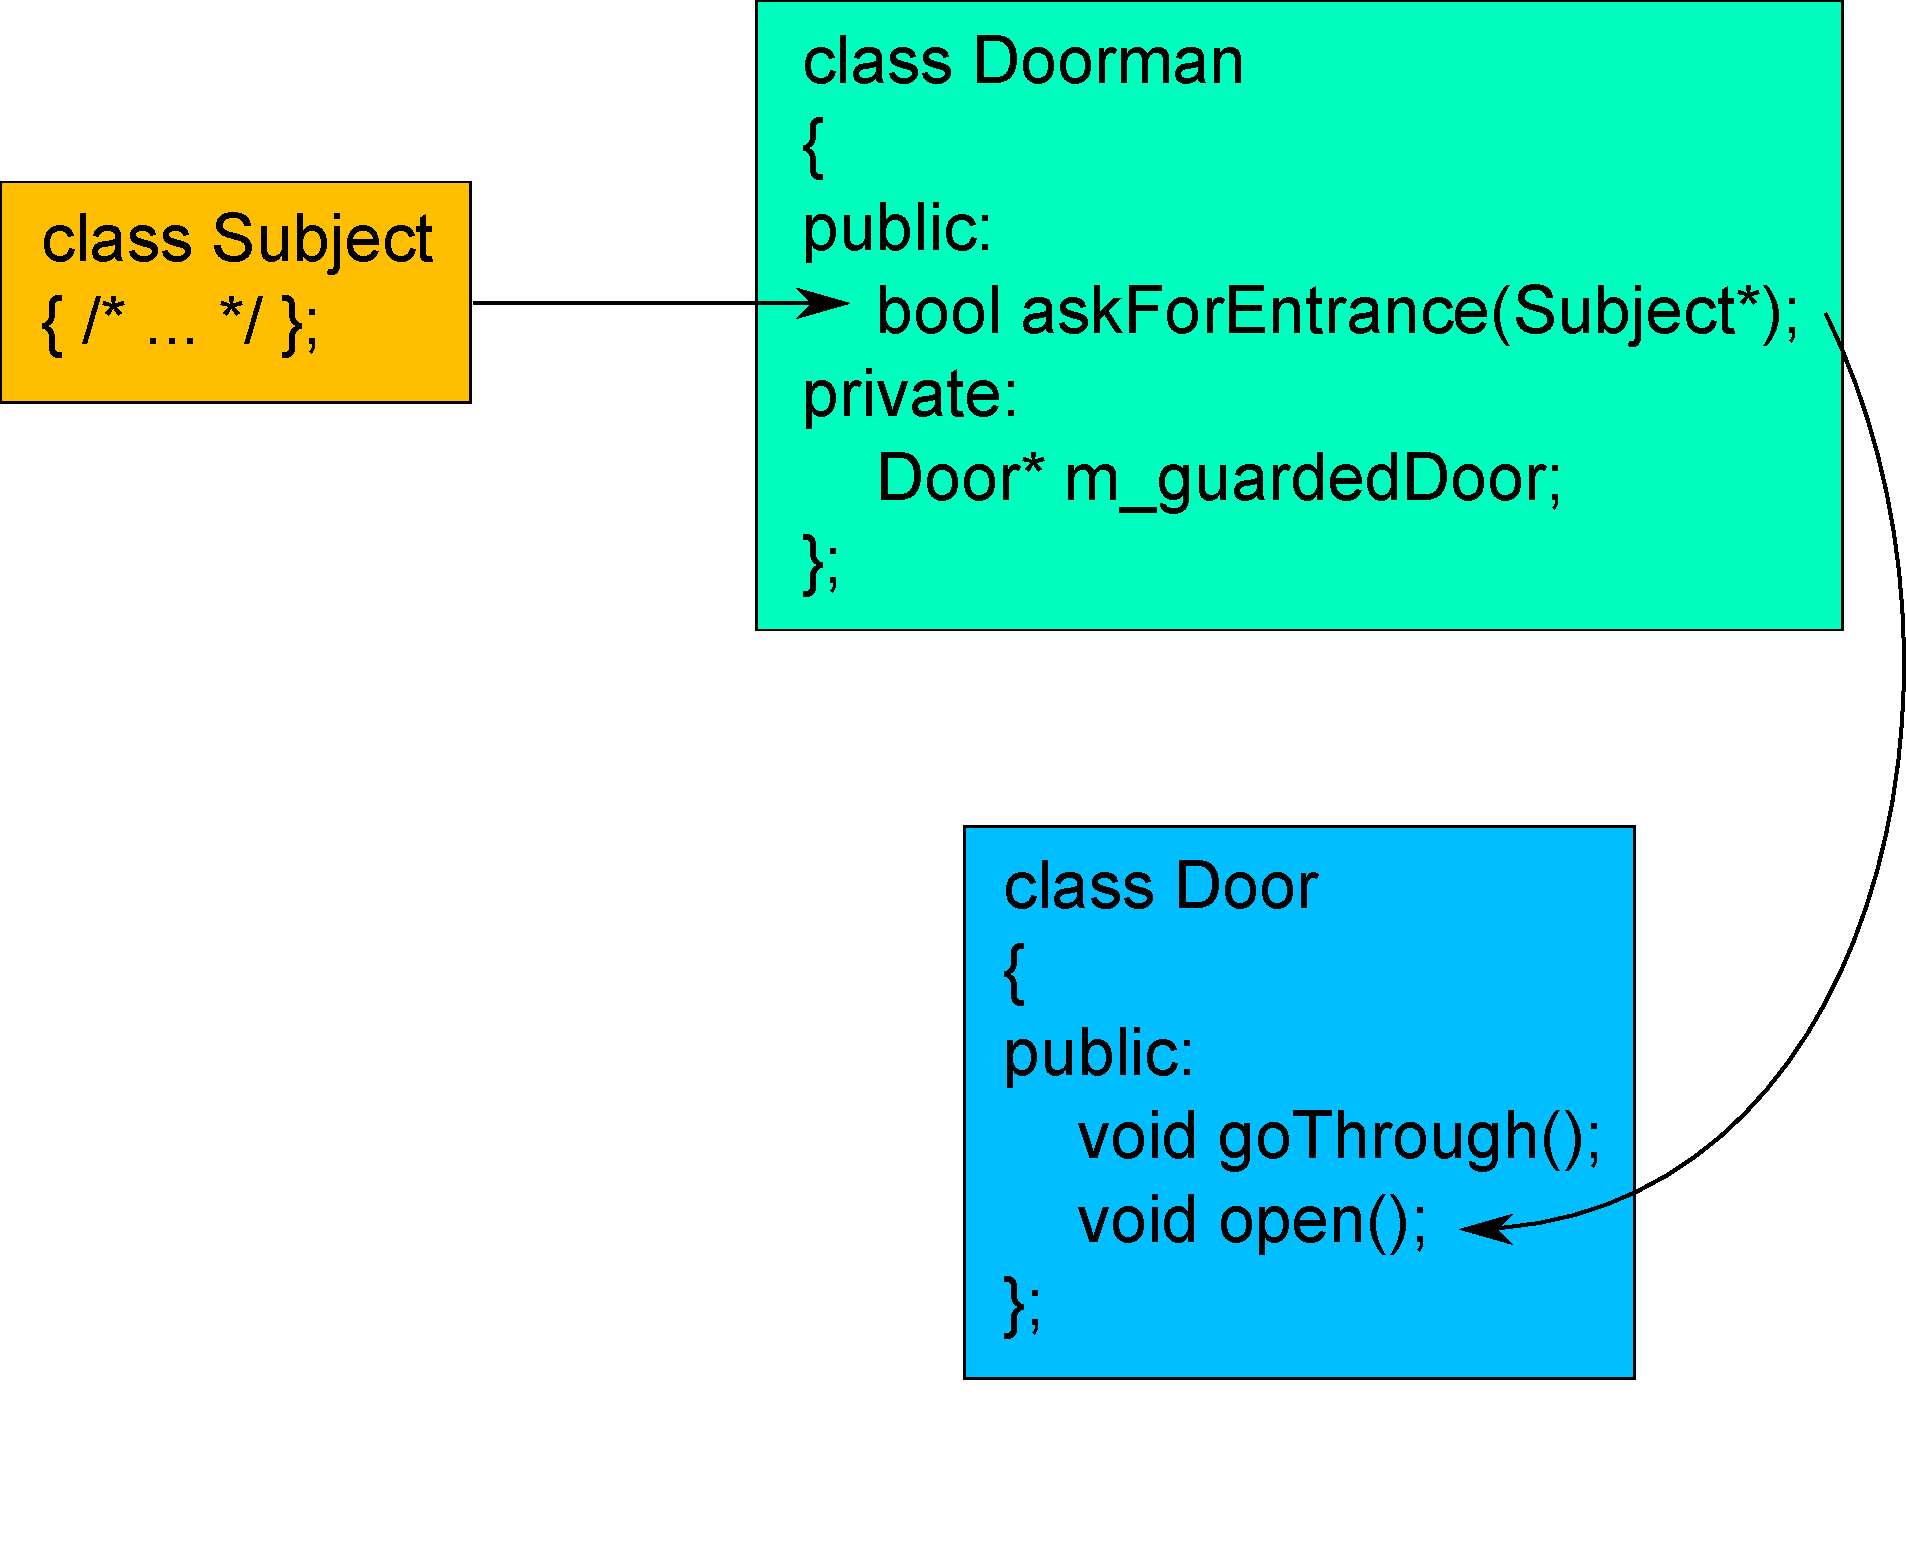
\includegraphics[height=0.75\textheight]{images/without-friendship-1} }
	\onslide*<+> { 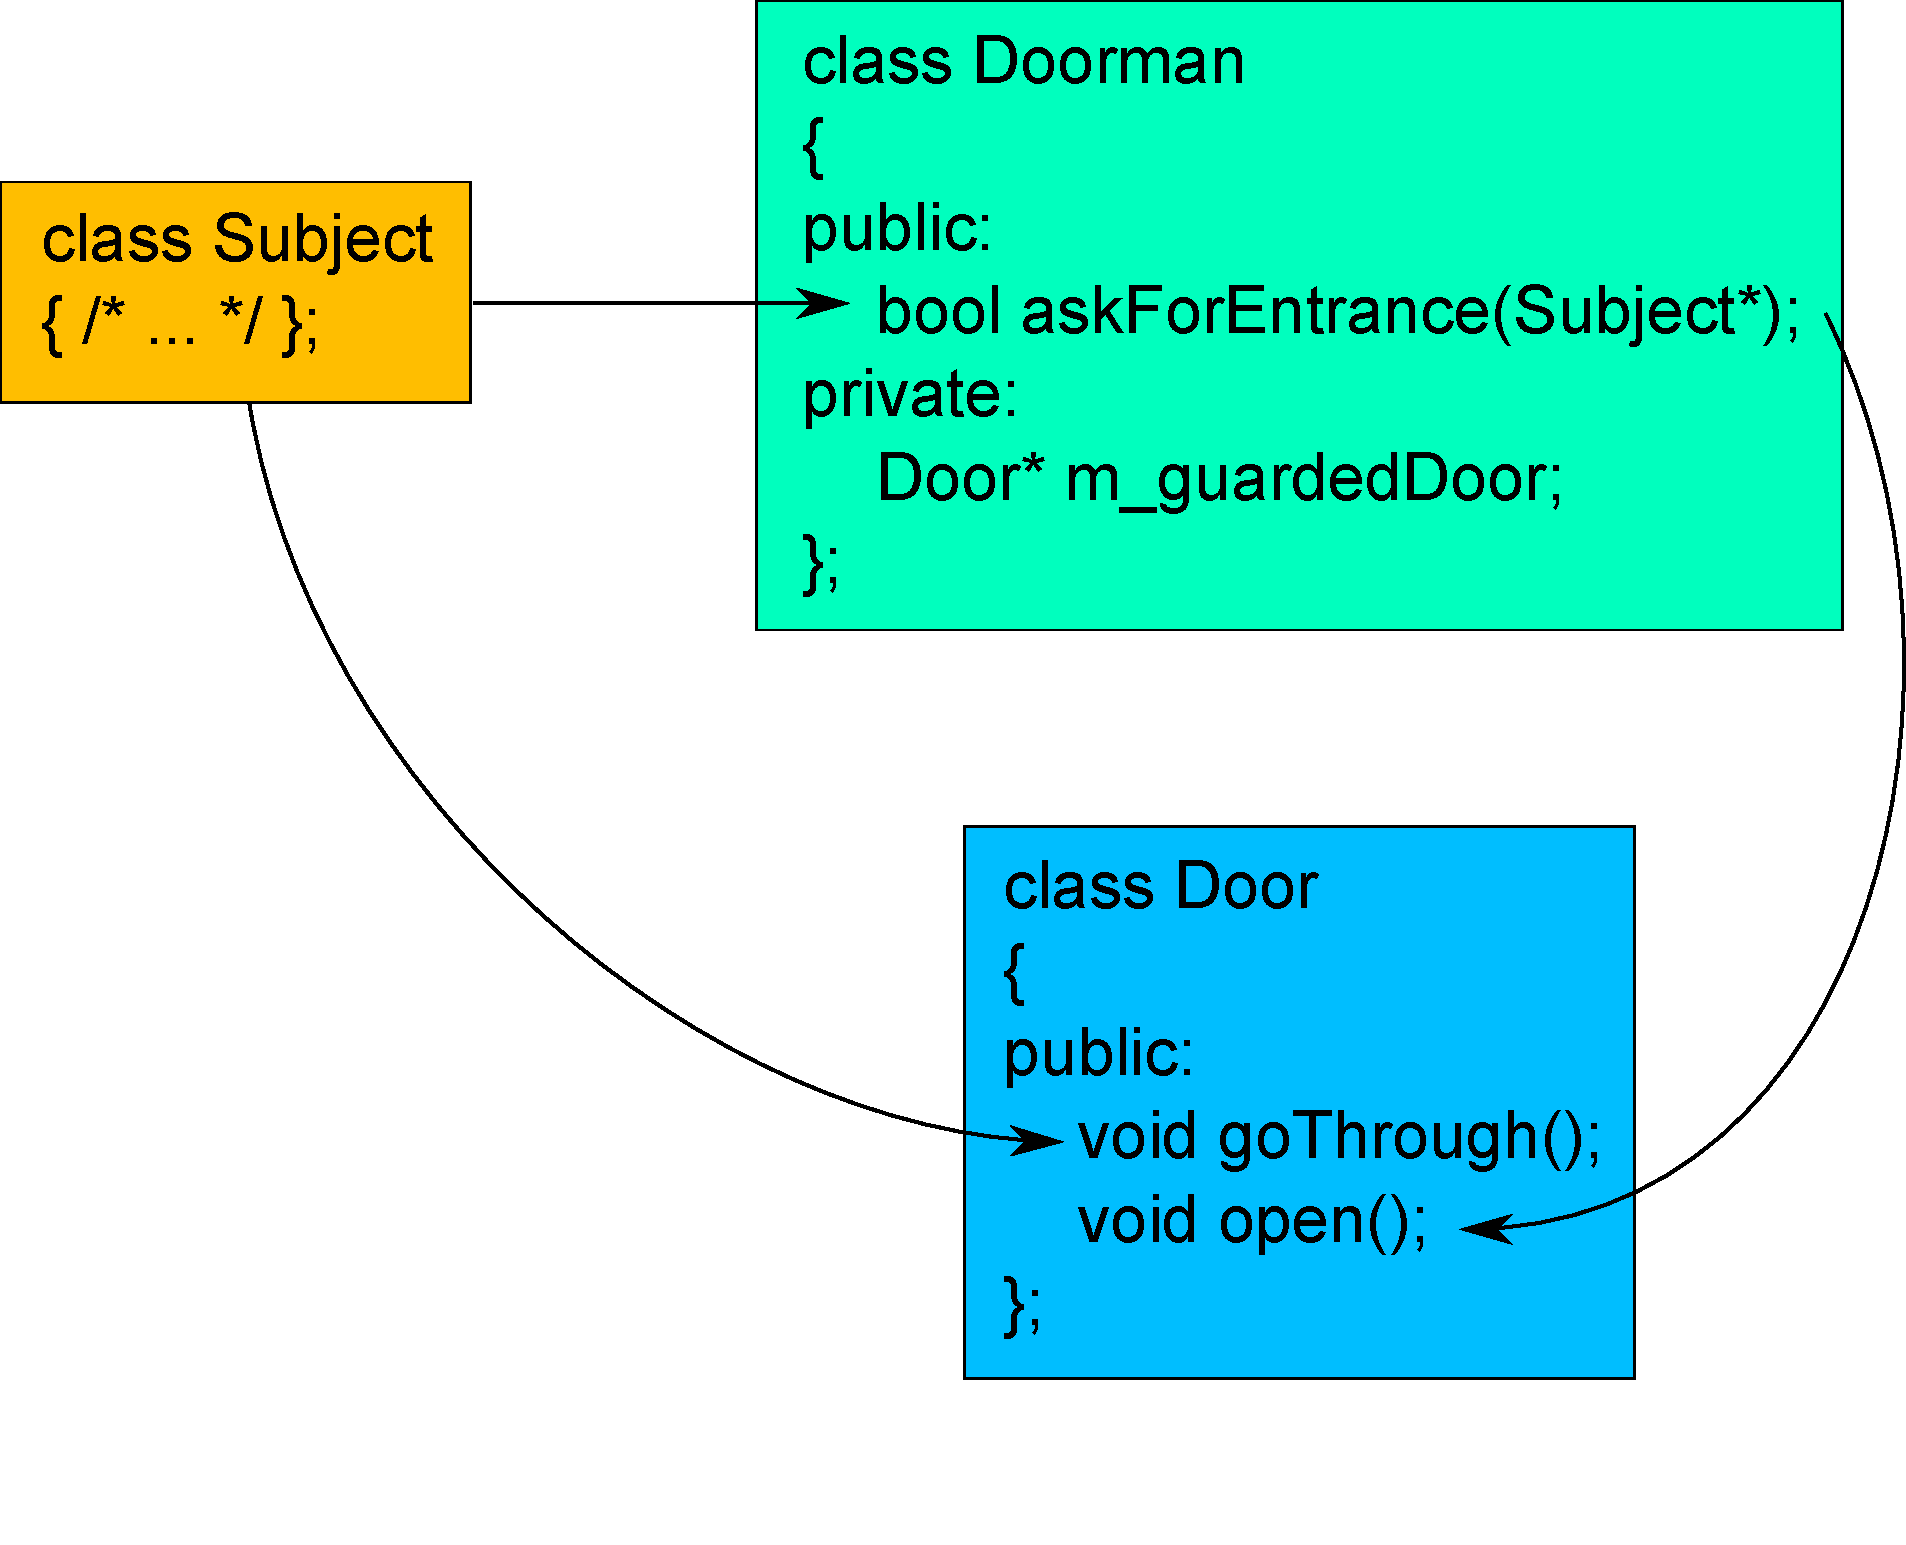
\includegraphics[height=0.75\textheight]{images/without-friendship} }
	\onslide*<+> { 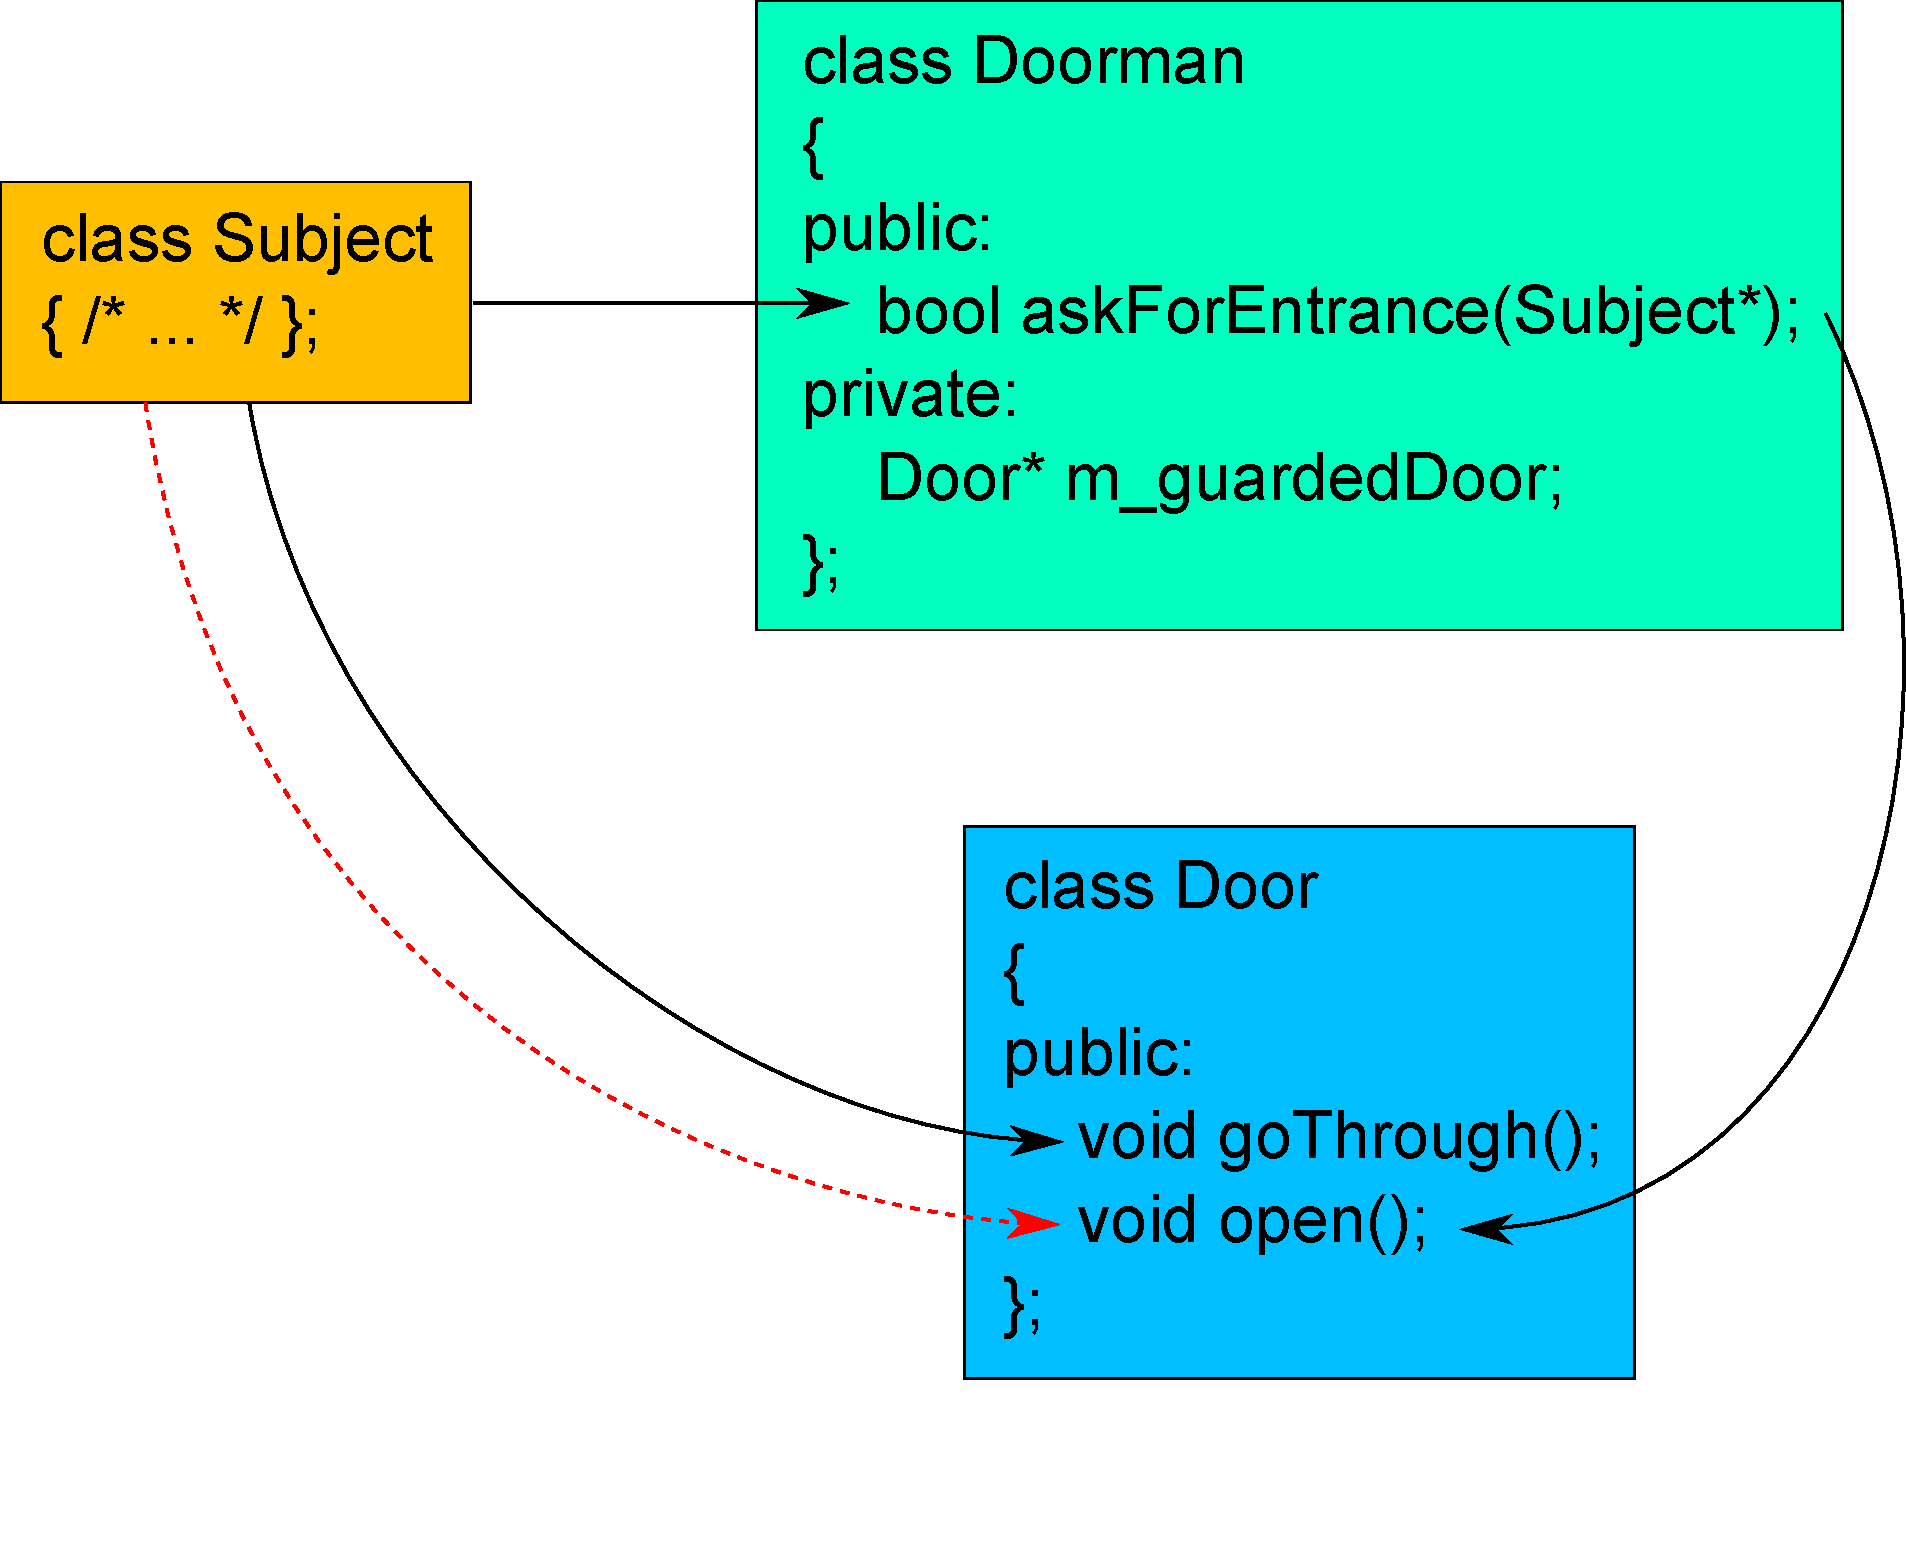
\includegraphics[height=0.75\textheight]{images/without-friendship-unauth} }
	\onslide*<+> { 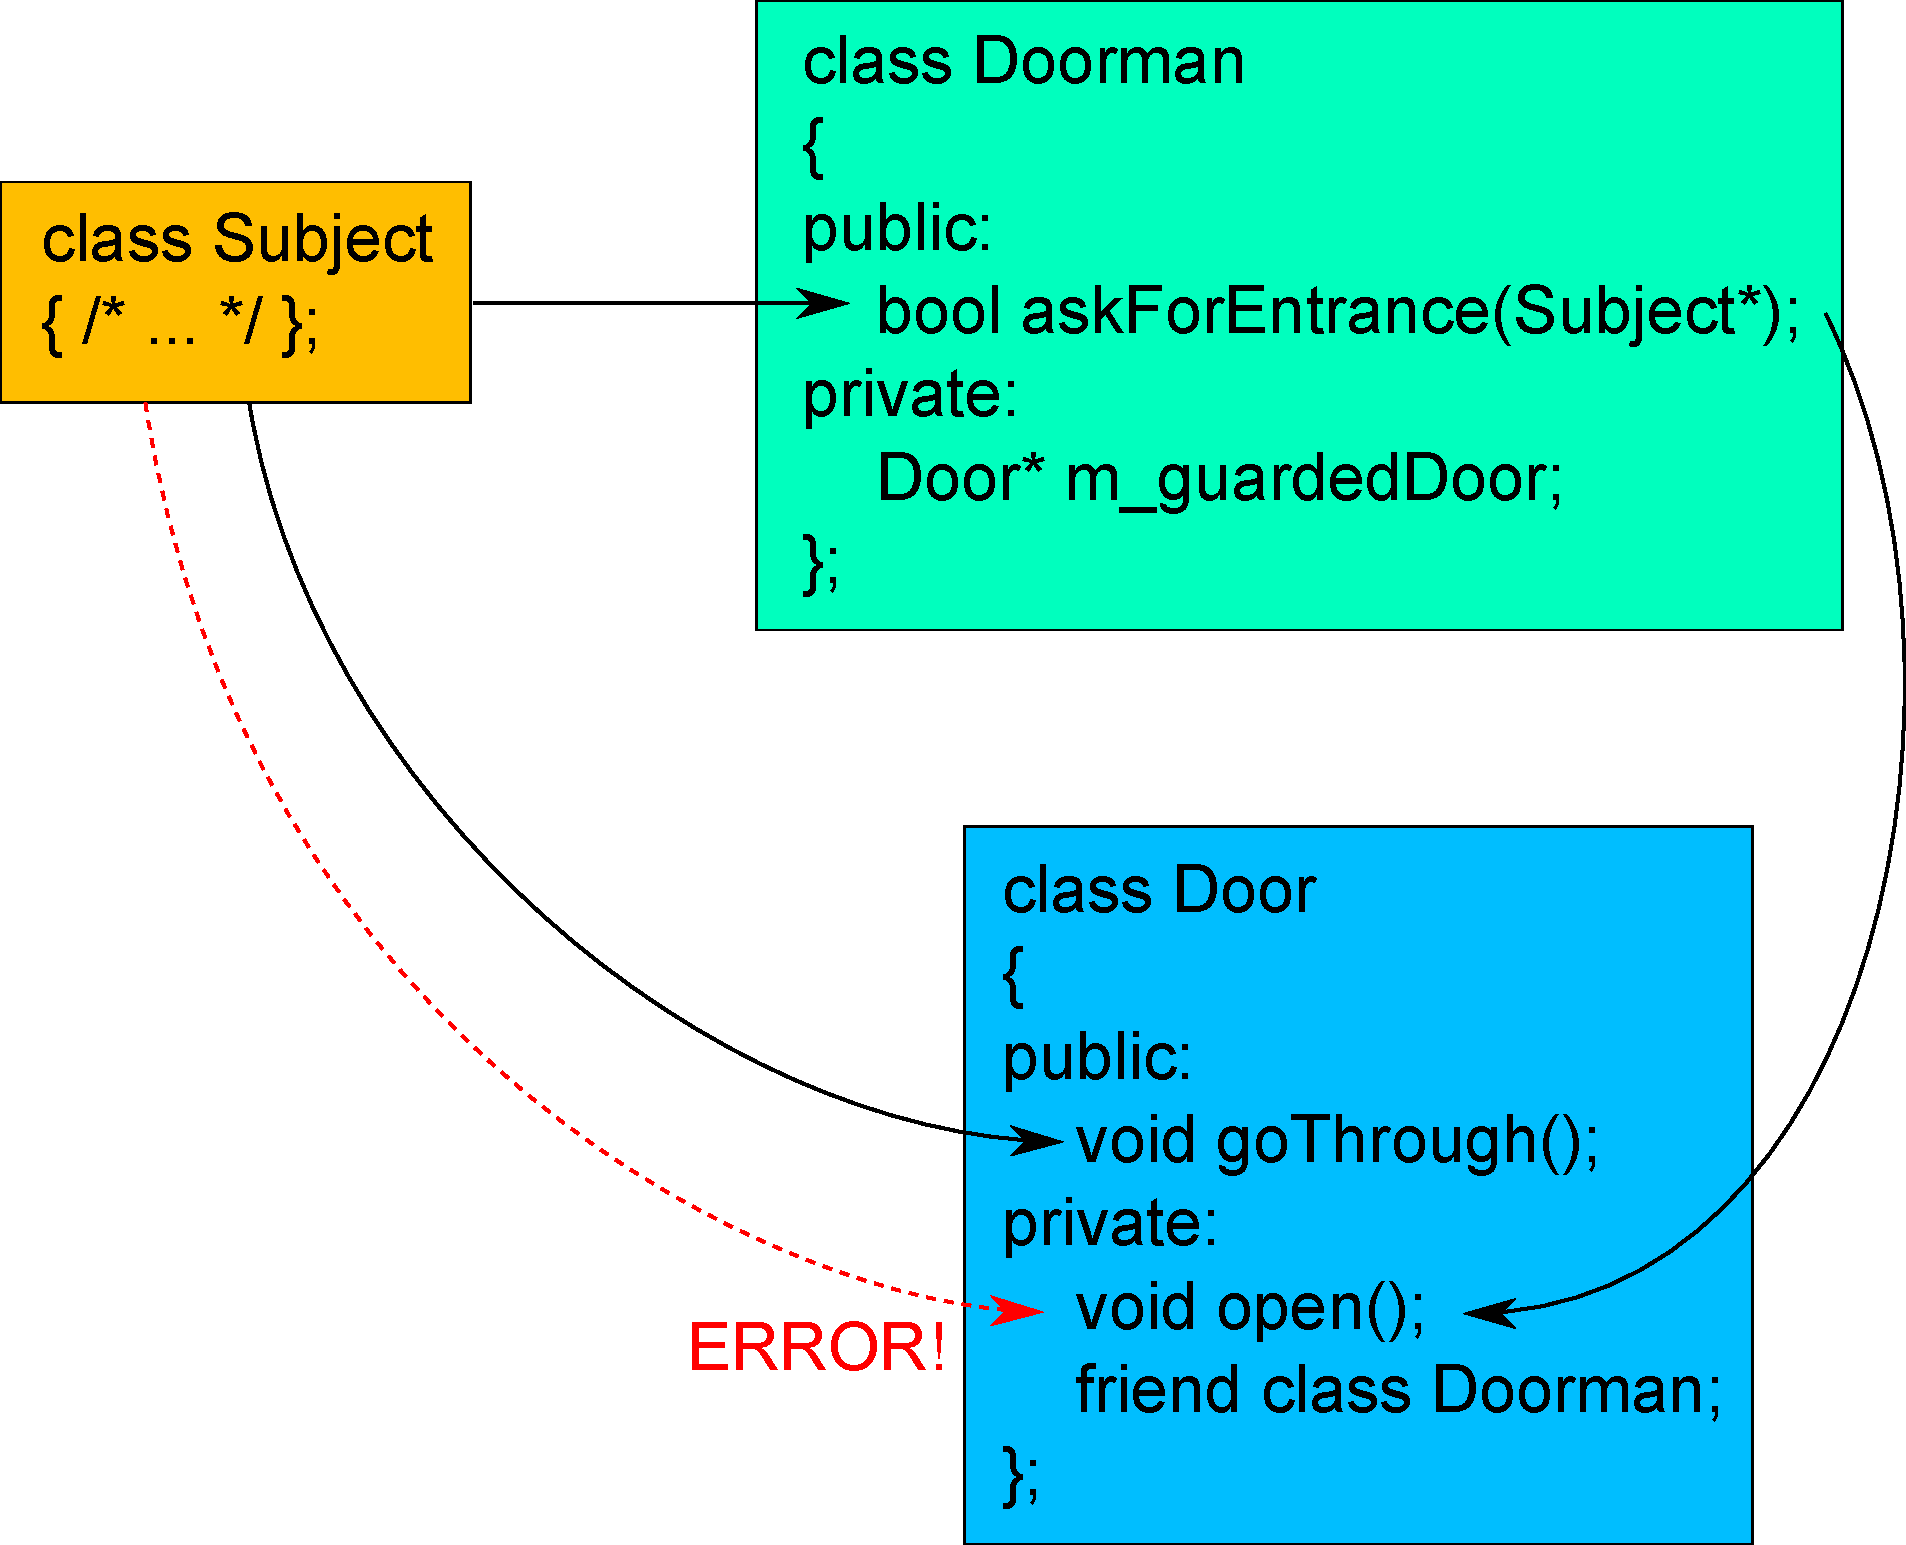
\includegraphics[height=0.75\textheight]{images/with-friendship} }
\end{frame}





\subsection{friend}

\begin{frame}[fragile]{Syntax}
	\begin{lstlisting}
struct B;
void globalFunc(B b);
struct A { void foo(B b); };

struct B {
    // public, private, protected or nothing at all
    friend class A;
    friend void globalFunc();
private:
    int m;
    void doInternal();
};
	\end{lstlisting}
	
	\pause
	
	\begin{block}{Syntax (Standard, 11.4)}
		Friendship gewährt man durch eine Deklaration in der Klassen-\emph{member-specification} mit \emph{friend-specifier} und für einen Typen mit \emph{elaborated-type-specifier} (7.1.5.3).
	\end{block}
\end{frame}


\begin{frame}[fragile]{Wirkung}
	Siehe Standard, 11.4.
	Hauptsächlich: man darf in member functions der befreundeten Klasse auf private member der Freundschaft-gewährenden Klasse zugreifen.
	
	\begin{block}{Beispiel}
		\begin{columns}[t]
			\column{0.55\textwidth}
			\begin{lstlisting}
struct B {
    friend class A;
    friend void globalFunc();
private:
    int m;
    void doInternal();
};
			\end{lstlisting}
			
			\column{0.45\textwidth}
			\begin{lstlisting}
void globalFunc(B b)
{
    b.doInternal();
}
void A::foo(B b)
{
    b.m = 42;
    b.doInternal();
}
			\end{lstlisting}
		\end{columns}
	\end{block}
\end{frame}


\begin{frame}{Hinweise}
	\begin{itemize}[<+->]
		\item Friendship wird nicht vererbt!
		\item Friendship ist nicht transitiv!
	\end{itemize}
\end{frame}

\section {Operatoren}

\subsection{Arten von Operatoren}

%\newcommand{\nov}[1]{\alert{#1}}
\newcommand{\cppop}[1]{ \texttt{#1} }
\newcommand{\pppp}{}


\begin{frame}[fragile]{Alle Operatoren in C++}
	\begin{block}{Alle Operatoren in C++}
		\begin{tabular}{r|l}
			memory			&	\verb|* & new new[] delete delete[]| \verb|sizeof|					\pause \\
			arithmetic		&	\verb!+ - * / % ^ & | ~ << >>!									\pause \\
			logic			&	\verb!&& ||! \verb|!|											\pause \\
			comparison		&	\verb|< > <= >= == !=|											\pause \\
			assignment		&	\verb!= += -= *= /= %= ^= &= |= >>= <<= ++ --!					\pause \\
			others			&	\verb|() [] ,|~~\verb|::|~~\verb|?:| \verb|typeid|				\pause \\
			member access	&	\verb|->* ->|~~\verb|.|~~\verb|.*|								\pause \\
		\end{tabular}
	\end{block}
	
	\vspace{2em}
	
	\onslide<+->
		42 overloadable operators + 4 unary forms
		
		Nicht überladbar: \verb|sizeof typeid . .* :: ?:|
\end{frame}


\begin{frame}[fragile]{Gruppiert nach Parameterzahl}
	\onslide<+->
		\begin{block}{Unäre Operatoren}
			\verb|! ++ --|~~sowie die unären Varianten von~~\verb|+ - * &|
		\end{block}
	
	\vspace{2em}
	
	\onslide<+->
		\begin{block}{Binäre Operatoren}
			(alle anderen)
		\end{block}
	
	\vspace{2em}
	
	\onslide<+->
		\begin{block}{Ternärer Operator}
			\verb|?:|
		\end{block}
\end{frame}




\subsection{Aufruf von Operatoren}

\begin{frame}[fragile]{Unäre Operatoren}
	\begin{block}{operator function invocation}
		For operator \cppop{@} and expression \cppop{a}:
		
		\vspace{1em}
		
		\begin{tabular}{l|l|l}
			expression	&	as member function	& as (global) function	\\
			\hline
			\cppop{@a}	&	\cppop{(a).operator@ ()}	&	\cppop{operator@ (a)}	\pause \\
			\cppop{a@}	&	\cppop{(a).operator@ (0)}	&	\cppop{operator@ (a, 0)}	\pause \\
			\cppop{a-\textgreater}	&	\cppop{(a).operator-\textgreater ()}	&	n/a \pause \\
		\end{tabular}
	\end{block}
	
	\vspace{1em}
	
	\onslide<+->
		\lstinputlisting[linerange={1-5}]{cpp-code/operator-invocation.cpp}
\end{frame}


\begin{frame}[fragile]{Binäre Operatoren}
	\begin{block}{operator function invocation}
		For operator \cppop{@} and expression \cppop{a}:
		
		\vspace{1em}
		
		\begin{tabular}{l|l|l}
			expression	&	as member function	& as (global) function	\\
			\hline
			\cppop{a@b}	&	\cppop{(a).operator@ (b)}	&	\cppop{operator@ (a, b)}	\pause \\
			\cppop{a=b}	&	\cppop{(a).operator= (b)}	&	n/a \pause \\
			\cppop{a[b]}	&	\cppop{(a).operator[] (b)}	&	n/a \pause \\
			\cppop{a(b)}	&	\cppop{(a).operator() (b)}	&	n/a \pause \\
		\end{tabular}
	\end{block}
	
	\vspace{1em}
	
	\onslide<+->
		\lstinputlisting[linerange={7-11}]{cpp-code/operator-invocation.cpp}
\end{frame}




\subsection{Zweck von Operator-Überladung}

\begin{frame}[fragile]{Wozu Operator-Überladung?}
	\begin{itemize}[<+->]
		\item intuitive Syntax z.B. für Matrizen \verb|A * B + C|
		\item Hinteranderausführen, etwa \verb|a + b + c| statt \verb|add(add(a, b), c)| oder \verb|a.add(b).add(c)|
		\item Syntax-Kompatibilität (z.B. Pointer und Smart-Pointer)
		\item Spezialfälle: address-of \cppop{\&} und class member access \cppop{-\textgreater} und assigment \cppop{=}
	\end{itemize}
\end{frame}




\subsection{Syntax}

\begin{frame}[fragile, b]{Einfache binäre Operatoren}
	\onslide*<+>
	{
		\begin{block}{\cppop{a.operator@ (b)}}
			\lstinputlisting[linerange={2-10}]{cpp-code/overloading-binary-operators.cpp}
		\end{block}
	}
	
	\onslide*<+>
	{
		Non-assigment operators und kein []
		
		\begin{block}{\cppop{operator@ (a, b)}}
			\lstinputlisting[linerange={14-22}]{cpp-code/overloading-binary-operators.cpp}
		\end{block}
	}
	
	\vspace{3em}
\end{frame}


\begin{frame}[fragile, b]{Binary assignment operators}
	\onslide*<+>
	{
		\begin{block}{a.operator@ (b)}
			\lstinputlisting[linerange={27-38}]{cpp-code/overloading-binary-operators.cpp}
		\end{block}
	}
	
	\onslide*<+>
	{
		Kein \cppop{[]} und kein \cppop{()}
		
		\begin{block}{operator@ (a, b)}
			\lstinputlisting[linerange={42-53}]{cpp-code/overloading-binary-operators.cpp}
		\end{block}
	}
	
	\vspace{1em}
\end{frame}


\begin{frame}{Unäre Operatoren: Präfix}
	\onslide*<+>
	{
		Non-assignment operators
		
		\begin{block}{a.operator@ ()}
			\lstinputlisting[linerange={2-9}]{cpp-code/overloading-unary-operators.cpp}
		\end{block}
	}
	
	\onslide*<+>
	{
		Non-assignment operators, kein -\textgreater
		
		\begin{block}{operator@ (a)}
			\lstinputlisting[linerange={13-20}]{cpp-code/overloading-unary-operators.cpp}
		\end{block}
	}
\end{frame}

\begin{frame}[fragile]{Unäre Operatoren: Suffix}
	Die einzigen unären Suffix-Operatoren sind \verb!++! und \verb!--!, also assigment-ops.
	
	\onslide*<+>
	{
		\begin{block}{a.operator@ (0)}
			\lstinputlisting[linerange={25-36}]{cpp-code/overloading-unary-operators.cpp}
		\end{block}
	}
	
	\onslide*<+>
	{
		\begin{block}{operator@ (a)}
			\lstinputlisting[linerange={40-51}]{cpp-code/overloading-unary-operators.cpp}
		\end{block}
	}
\end{frame}




\subsection{member functions oder non-member functions?}

\begin{frame}[fragile]{Fälle ohne Wahlmöglichkeit}
	Bei diesen Operatoren gibt es nur die member-function-Variante: \verb!= [] () ->!
	
	\pause
	\vspace{1em}
	
	Bei allen anderen Operatoren hat man die Wahl.
	
	Einschränkung: operator function invocation
	\begin{lstlisting}
		#include <ostream>
		#include <iostream>
		
		using namespace std;
		extern ostream cout;	// definition of the cout object according to 27.3
		
		MyClass p { /* ... */ };
		
		std::ostream& operator <<(ostream& o, MyClass p)
		{ /* ... */ return o;}
	\end{lstlisting}
\end{frame}

\begin{frame}[fragile]{Fälle mit Wahlmöglichkeit}
	Habe keine guten Entscheidungshilfen gefunden!
	
	\vspace{1em}
	
	Bemerkung:\\
	Zwecks Symmetrie nimmt man meist die Variante mit der non-member function:
	\begin{lstlisting}
		class MyInt;
		MyInt operator+ (MyInt, int);
		MyInt operator+ (int, MyInt);
		
		class MyInt {
		    friend MyInt operator+ (MyInt, int);
		    // MyInt operator +(MyInt int);
		    friend MyInt operator+ (int, MyInt);
		    // n/a
		    
		private:
		    int m;
		};
	\end{lstlisting}
\end{frame}




\subsection{Wichtige Hinweise}

\begin{frame}[fragile]{Self-assignment}
	\onslide*<+>
	{
		\lstinputlisting[linerange={1-14, 32-34}]{cpp-code/self-assignment.cpp}
	}
		
	\onslide*<+>
	{
		\lstinputlisting[linerange={17-30, 32-34}]{cpp-code/self-assignment.cpp}
	}
\end{frame}

\begin{frame}[fragile]{Weitere Hinweise}
	\url{http://www.parashift.com/c++-faq-lite/operator-overloading.html#faq-13.9}
	
	\vspace{2em}
	
	\begin{itemize}[<+->]
		\item operator overloading ist nicht dafür da, dem class designer das Leben einfacher zu machen, sondern dem Nutzer einer Klasse!
		\item Operatoren sollten intuitive und eindeutige Bedeutung haben
		\item Identitäten sollten erhalten bleiben, z.B. \verb|x == x + y - y|
		\item manche Operatoren sollten den ersten Operanden verändern, z.B. \verb|= += *=|
		\item manche aber eben nicht, z.B. \verb|+ * /|
	\end{itemize}
\end{frame}


\section{Praxis}
\begin{frame}[fragile]{Praxis!}
	\begin{itemize}
		\item Aufgabe 1: Schachprogramm bis nächste Woche fertig machen
	\end{itemize}
	\ \\
	\ \\
	\large{\url{https://github.com/kit-cpp-workshop/workshop-ss12-06}} \\
	\ \\
	Aufgabenbeschreibungen und Hinweise: Siehe \verb|README.md|

\end{frame}


\end{document}
